\section{Log of \ref{sec:WBSTaskRepresentation} triple}

Task atomico, non suddiviso in sottotask.
\subsection{22/12/2009}
\paragraph{Esempio 1}
\paragraph{input}
\begin{figure}
\centering
\includegraphics{/../../tests/TEST WBS/4.1/4.1 - 1/Esempio 1/input.png}
\includegraphics{/../../tests/TEST WBS/4.1/4.1 - 1/Esempio 1/input - actual.png}
\end{figure}
\paragraph{environment}
\begin{figure}
\centering
\includegraphics{/../../tests/TEST WBS/4.1/4.1 - 1/Esempio 1/environment.png}
\end{figure}
\paragraph{esito}
\begin{figure}
\centering

\includegraphics{/../../tests/TEST WBS/4.1/4.1 - 1/Esempio 1/output.png}
\end{figure}

\paragraph{Esempio 2}
\paragraph{input}
\begin{figure}
\centering
\includegraphics{/../../tests/TEST WBS/4.1/4.1 - 1/Esempio 2/input.png}
\includegraphics{/../../tests/TEST WBS/4.1/4.1 - 1/Esempio 2/input - actual.png}
\end{figure}
\paragraph{environment}
\begin{figure}
\centering
\includegraphics{/../../tests/TEST WBS/4.1/4.1 - 1/Esempio 2/environment.png}
\end{figure}
\paragraph{esito}
\begin{figure}
\centering

\includegraphics{/../../tests/TEST WBS/4.1/4.1 - 1/Esempio 2/output.png}
\end{figure}

\paragraph{Esempio 3}
\paragraph{input}
\begin{figure}
\centering
\includegraphics{/../../tests/TEST WBS/4.1/4.1 - 1/Esempio 3/input.png}
\includegraphics{/../../tests/TEST WBS/4.1/4.1 - 1/Esempio 3/input - actual.png}
\end{figure}
\paragraph{environment}
\begin{figure}
\centering
\includegraphics{/../../tests/TEST WBS/4.1/4.1 - 1/Esempio 3/environment.png}
\end{figure}
\paragraph{esito}
\begin{figure}
\centering

\includegraphics{/../../tests/TEST WBS/4.1/4.1 - 1/Esempio 3/output.png}
\end{figure}
